\chapter{Testing}
\label{chap:num_7}

The following section will provide an overview of testing practices followed during the implementation described in \autoref{chap:num_5}. The chapter will start by describing the preliminary technologies used for implementing automated testing, integration, and delivery pipelines as well as libraries used for unit testing of TypeScript base \lpas{} package.

\section{Technologies used}

The main development stack consisted of the following technologies: 
\begin{itemize}
    \item \textit{\texttt{ava.js}} \footnote{\url{https://github.com/avajs/ava}} is a \texttt{Node.js} unit testing library. It provides a clean and minimalistic syntax for writing tests, concurrent tests execution, includes TypeScript definitions and supports asyncronous functions. All of the aforementioned factors were considered when choosing this package as main unit testing library for \lpas{} package.
    
    \item \textit{\texttt{tslint}} \footnote{\url{https://palantir.github.io/tslint/}} is an extensible static analysis tool that checks TypeScript code for readability, maintainability, and functionality errors. It is widely supported across modern editors and build systems and can be customized with your own lint rules, configurations, and formatters.
    
    \item \textit{\texttt{istanbul.js}} \footnote{\url{https://istanbul.js.org/}} is a code coverage analyzer. It checks ES2015+ JavaScript code with line counters providing a very extensive overview of all classes and their coverage.
    
    \item \textit{Travis CI} \footnote{\url{https://travis-ci.org/}} is a hosted, distributed continuous integration service used to build and test software projects hosted at GitHub. Travis CI is used to check that newly committed code does not break the build and, consequently, the system. This ensures that developers are not disrupted and that the system remains stable. It is also able to run available automated tests to check further that the system is working correctly, even if the build isn't broken.

    \item \textit{Renovate} \footnote{\url{https://docs.renovatebot.com/}} is an automated dependency updater. Multi-platform and multi-language. Due to various dependencies used in the \emph{frontend} web component, it is crucial to keep the project up to date with the latest stable software releases. Renovate is set up and being triggered using Github Webhooks each weekend to check for updates in \texttt{package.json} and make a pull request to \texttt{master} and \texttt{develop} branches if any available.

    \item \textit{Codecov} \footnote{\url{https://codecov.io/}} is an automated code review tool that allows developers to improve code quality and monitor technical debt. Codecov automates code reviews and monitors code quality on every commit and pull request. It reports back the impact of every commit or pull request in new issues concerning code style, best practices, security, and many others. It monitors changes in code coverage, code duplication, and code complexity. It allows developers to save time in code reviews, tackle issues efficiently, and overall makes the system maintainability much easier.
    
    \item \textit{Slack} \footnote{\url{https://slack.com/}} a cloud-based proprietary instant messaging platform developed by Slack Technologies. The platform was used for automated notifications from GitHub and Travis-CI to report the states of executed CI and CD pipelines and for communication with the \lpa{} developers.
\end{itemize} 

\section{Unit testing}

Every class in \lpas{} package was unit tested using the ava.js library. The convention used required in-place creation of a file with ava.js tests definitions named identical to a \texttt{.ts} file to be tested but with \texttt{.spec.} prefix appended before the file extension. The listing on \autoref{lst:unit_testing_create_resource} demonstrates the example serial ava.js test executed in order. The asynchronous \textit{createResource} can be reused in multiple ava.js tests improving code reusability while writing new tests.

\begin{listing}[H]    
\begin{minted}[breaklines,frame=single,framerule=1pt]{javascript}
async function createResource(t: any, input: any, expected: any): Promise<any> {
  const result = await StorageFileManager.createResource(input);
  logger.info(result.text());
  t.is(result.status, expected);
}

test.serial(
  'createFolderResource',
  createResource,
  folderConfigurationResource,
  201
);
\end{minted}
\caption{An example of a reusable asynchronous test chunk and single serial ava.js test for \textit{createResource()} method from \textit{FileManager} abstraction in \lpas{} package.} 
\label{lst:unit_testing_create_resource}
\end{listing}

The istanbul.js JavaScript coverage library has integration with ava.js. The official command-line interface of istanbul.js, called \texttt{nyc} is used to invoke the unit tests to both run the tests and visualize the test results in the terminal in a convenient format.

Unit tests are automatically executed on every push to any remote branch on \lpas{} package repository. More details on executing the unit tests in automated pipelines are provided in next section.

\section{Continious Integration and Delivery}

The section will provide details on implementing automated integration and delivery pipelines using Travis CI.
The terms Continuous Integration stands for a development practice that requires a developer to integrate his latest commits to a shared repository regularly. On the other hand, the name Continuous Delivery stands for an ability to deliver code changes of any type to production in a quick, safe, and automated way. Both of the practices were taken into consideration while implementing the \lpas{} package. 

\subsection{Using Travis CI}

Travis CI was used in pairs with the GitHub platform. As the first step, the service was connected with \lpas{} package GitHub repository using Webhooks \footnote{\url{https://en.wikipedia.org/wiki/Webhook}}. Secondly, a special \texttt{.travis.yml} the configuration file was added to all branches of \lpas{} repository. The configuration file defined the integration and delivery pipelines to be executed inside Travis CI. Using a special feature called \textit{build matrix}, the \lpas{} was set to be unit tested automatically in concurrent manner on both \texttt{Node.js v10.x} and \texttt{Node.js v12.x}. 

The branch protection rules were also applied to \texttt{dev} and \texttt{master} branches on \lpas{} repository. The additional step in Travis CI pipeline configuration was added for \texttt{master} branch. Every push on remote \texttt{master} on \lpas{} repository also involves deployment to \texttt{npm}. Failed build states are propagated into a special slack channel in \lpa{} Slack workspace, channel is dedicated specifically for reporting CI and CD pipeline execution statuses for all branches on \lpas{} repo.

\section{Integration testing in \lpa{}}

The diagram on \autoref{chap:introduction} is a detail demonstration of how \lpa{} and \lpa{} package are integration tested in automated and semi-automated manner. It is important to note that the example on diagram considers a case when \lpas{} developer merges changes into \texttt{master} branch of \lpas{} package.

\begin{figure}[h]
\centering
\fcolorbox{black}{white}{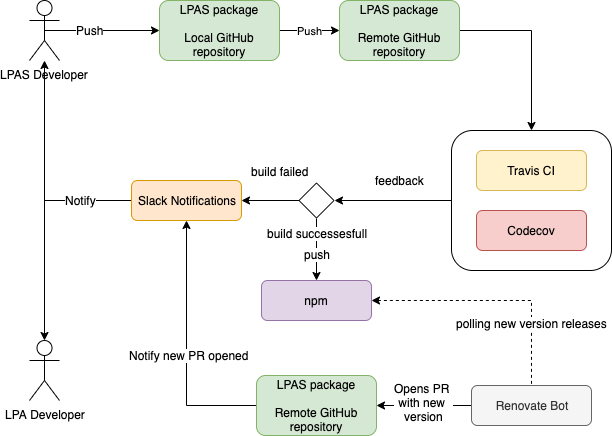
\includegraphics[width=0.8\linewidth]{lpas_ci_integration.png}}
\caption{A detailed overview of CI and CD pipeline interaction for \lpa{} and \lpas{}.}
\label{fig:lpas_ci_integration}
\end{figure}

The operational flow can be described as follows:
\begin{enumerate}
    \item \textit{\lpas{} developer pushes code to \texttt{master} branch}, the code is pushed to a remote GitHub repository. This triggers the Travis CI and Codecov reviews via Webhooks.
    \item \textit{Travis CI evaluates the results of pipeline}. If result is successfull it automaticall pushes the new version into npm and updates the static documentation for TypeScript classes. If failed, then the \lpas{} developer is notified on Slack channel with a report on why the pipeline is failed.
    \item \textit{Renovate bot polls for new \lpas{} releases}, the Renovate bot instance attached to \lpa{} platform repository periodaclly polls \texttt{npm} and opens a Pull Request with new \lpas{} package to \lpa{} platform on a branch called \texttt{dependency-updates}. 
    \item \textit{The \lpa{} developer is notified via Slack}. When a Pull Request into \lpa{} codebase is opened by Renovate, it notifies the \lpa{} developer via Slack to review the Pull Request and merge new release of \lpas{} package.
\end{enumerate} 